\begin{frame}
    \frametitle{Алгоритм постановки задачи в расписание}
    {
        \tiny
        \ctikzfig{schedule-time-diagram}
    }
    Проблема: даже в при максимально плотном установлении задач в конец расписания, образуются "пробелы" в расписании, в которые возможно установить работы без нарушения его целостности.
\end{frame}

% \begin{frame}
%     \frametitle{Алгоритм постановки задачи в расписание}
%     \begin{enumerate}
%         \item При постановке задачи на процессор рассматриваются все ее предшественники, вычисляются времена их завершения на своих процессорах
%         \item  В случае если они находятся не на том же процессоре на который мы пытаемся поставить задачу, прибавляем к ним время передачи
%         \item Из получившегося набора берется максимум - "зависимость по задачам"
%         \item Рассматриваются все пропуски на процессоре, находящиеся после "зависимости по задачам", и, если длительность какого-либо пропуска больше или равна времени выполнения данной задачи на процессоре - задача помещается в пропуск.
%         \item Если данная процедура дырку не нашла - задача помещается в конец
%     \end{enumerate}
% \end{frame}

\begin{frame}
    \frametitle{Алгоритм постановки задачи в расписание}
    \begin{columns}
        \begin{column}{0.5\textwidth}
            \begin{figure}
                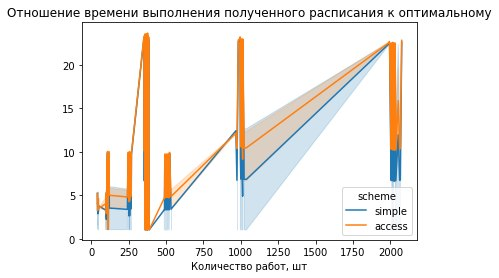
\includegraphics[width=\linewidth]{imgs/schedule_time_no_hp.jpg}
                \caption*{Без оптимизированной постановки}
            \end{figure}
        \end{column}
        \begin{column}{0.5\textwidth}
            \begin{figure}
                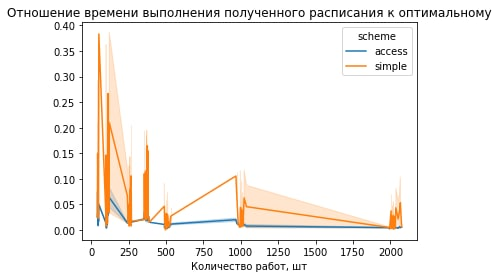
\includegraphics[width=\linewidth]{imgs/schedule_time_with_hp.jpg}
                \caption*{С оптимизированной постановкой}
            \end{figure}
        \end{column}
    \end{columns}
\end{frame}

\begin{frame}
    \frametitle{METIS и алгоритмы разбиения графов}
    \begin{figure}
        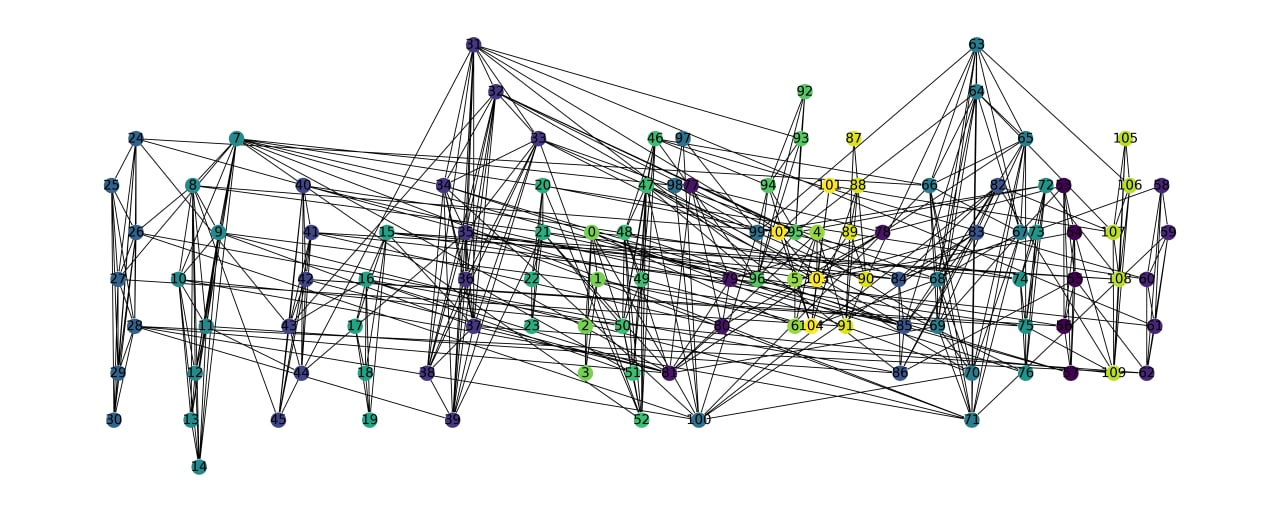
\includegraphics[width=\linewidth]{imgs/graph_part.jpg}
    \end{figure}
\end{frame}

\begin{frame}
    \frametitle{METIS и алгоритмы разбиения графов. Взвешенность.}
    \begin{figure}
        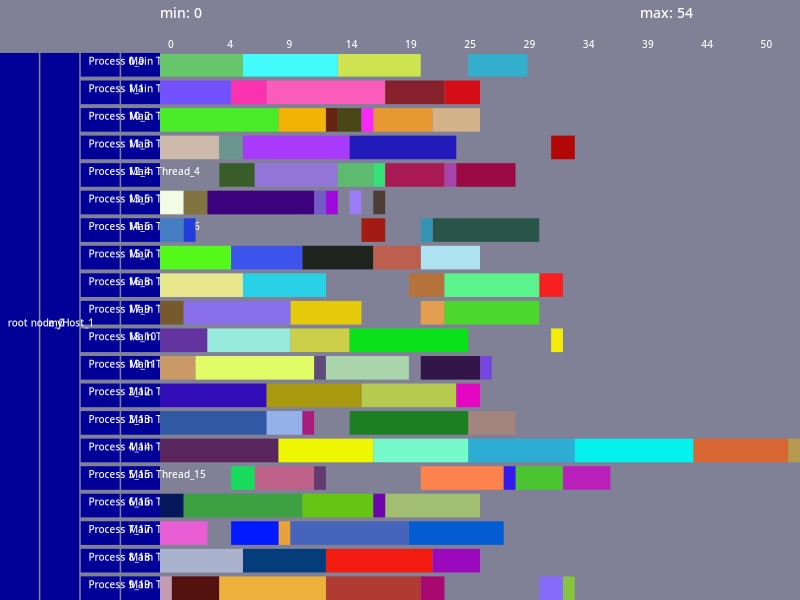
\includegraphics[height=0.8\textheight]{imgs/schedule_no_balanced.jpg}
    \end{figure}
\end{frame}

\begin{frame}
    \frametitle{METIS и алгоритмы разбиения графов. Взвешенность.}
    \begin{figure}
        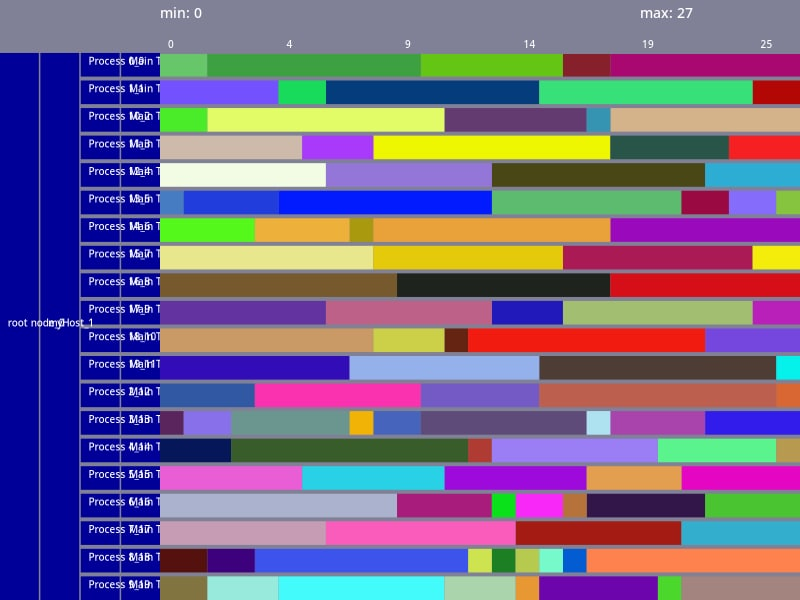
\includegraphics[height=0.8\textheight]{imgs/schedule_balanced.jpg}
    \end{figure}
\end{frame}

\begin{frame}
    \frametitle{METIS и алгоритмы разбиения графов. Взвешенность.}
    \begin{figure}
        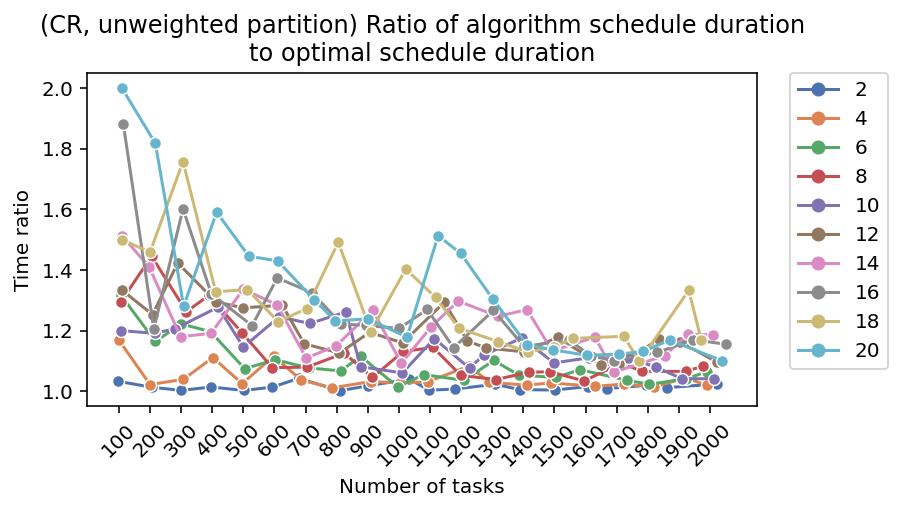
\includegraphics[width=0.8\linewidth]{imgs/unweighted_ratio.png}
    \end{figure}
\end{frame}

\begin{frame}
    \frametitle{METIS и алгоритмы разбиения графов. Взвешенность.}
    \begin{figure}
        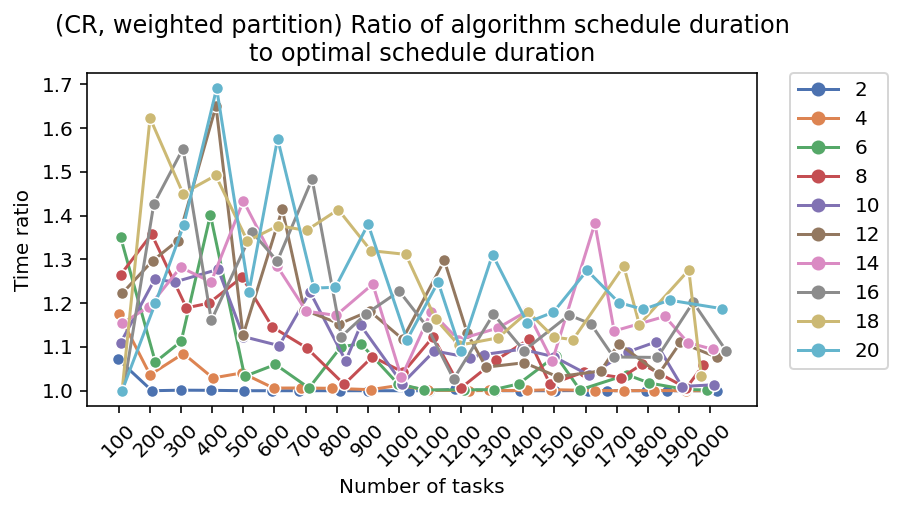
\includegraphics[width=0.8\linewidth]{imgs/weighted_ratio.png}
    \end{figure}
\end{frame}